\chapter{Herleitungen und Ausführungen}
%\addtocontents{toc}{\protect\setcounter{tocdepth}{0}}%  Sections tauchen ab hier nicht mehr im Inhaltsverzeichnis auf.
\section{Koordinatensysteme der lokalen und globalen Eigenlokalisierung} \label{app:kos}
Zur Darstellung eines optimierten Einsatzes der beiden Lokalisierungsmethoden und der entsprechenden Koordinatensysteme, s.\ \abb{fig:KOS}, soll das automatische Ausweichen auf einen unmittelbar vor dem Fahrzeug die Fahrbahn betretenden Fußgänger herangezogen werden. Dieser sei vom Videosensor erkannt, sodass seine Position 
%und Bewegunsrichtung\footnote{Optischer Fluss, s. Dang} 
in den Sensorkoordinaten der Kamera zur Verfügung steht, s.\ \emph{Sensorfeste Koordinaten} in Abb.\,\ref{fig:KOS}. Da die Einbauposition und -ausrichtung des Sensors relativ zu einem fahrzeugfesten Referenzpunkt bekannt sind (dies ist Aufgabe der Sensorkalibrierung), kann die Fußgängerposition aus den Sensorkoordinaten mittels der inversen Transformation von $T_\text{sens}$ in fahrzeugfeste Koordinaten umgerechnet werden. Entspricht der Ursprung der fahrzeugfesten Koordinaten noch nicht dem Bezugspunkt der Koppelnavigation (\emph{Fahrzeugfeste Koordinaten II}, s. Abb.\,\ref{fig:KOS} links unten), so muss die Fußgängerposition in das \emph{Fahrzeugfeste Koordinatensystem I} transformiert werden; ansonsten entfällt dieser Zwischenschritt. \\
Die Koppelnavigation liefert nun in jedem Zeitschritt die aktuelle Koordinatentransformation $T_\text{lok}(t)$, sodass deren Inverse aus der zuvor berechneten fahrzeugfesten Fußgängerposition die dazugehörigen ortsfesten Koordinaten mit weitgehend\footnote{Aufgrund numerischer Ungenauigkeiten von großen Fließkommazahlen sollte sich der Ursprung immer in der Nähe des Fahrzeugs befinden, was beispielsweise durch \emph{wrapping} der Koordinaten mittels Modulo-Operator \cite{himmelsbach2008lidar} sichergestellt wird.} frei festgelegtem Ursprung liefert. 
Das Ergebnis ist die Fußgängerposition des aktuellen Zeitpunkts in ortsfesten Koordinaten, welche mit verstreichender Zeit aufgrund des Drifts in $T_\text{lok}(t)$ \emph{langsam} an Genauigkeit verliert. \\
Zur Anpassung der Endausrichtung und -krümmung des Ausweichmanövers an den (für die Kamera nicht genau auszumachenden) Straßenverlauf soll nun eine digitale Straßenkarte hinzugezogen werden. Da sie absolut referenziert ist, d.h.\ in weltfesten Koordinaten erstellt wurde, muss der interessante Straßenverlauf in die ortsfesten Koordinaten transformiert werden, wo die Manöverplanung erfolgen soll. Wie zuvor beschrieben ist für diesen Schritt eine absolute Positionierung  des Fahrzeugs erforderlich, etwa über GPS. Bei bekannter Antennenposition am Fahrzeug kann hierdurch die aktuelle Transformationsvorschrift $T_\text{glob}(t)$ errechnet werden, s.\ auch Abb.\,\ref{fig:Odo_drift}, welche schließlich  den Straßenverlauf der Manöverberechnung in den ortsfesten Koordinaten zur Verfügung stellt und somit der Ausweichvorgang geplant und stabilisiert werden kann.

\begin{figure}[h]
\newcommand{\smallsize}{.85}
	\psfrag{0}[cc][cc][1.0]{\parbox[c]{7cm}{\begin{center} Weltfeste \\ Koordinaten \end{center}}}
	\psfrag{1}[cc][cc][1.0]{\parbox[c]{7cm}{\begin{center} Ortsfeste \\ Koordinaten \end{center}}}
	\psfrag{2}[cc][cc][1.0]{\parbox[c]{7cm}{\begin{center} Fahrezeugfeste \\ Koordinaten I \end{center}}}
	\psfrag{3}[cc][cc][1.0]{\parbox[c]{7cm}{\begin{center} Sensorfeste \\ Koordinaten \end{center}}}
	\psfrag{4}[cc][cc][1.0]{\parbox[c]{7cm}{\begin{center} Fahrzeugfeste \\ Koordinaten II \end{center}}}
	\psfrag{a}[lc][lc][1.0]{$T_\text{glob}(t)$}
	\psfrag{b}[lc][lc][1.0]{$T_\text{lok}(t)$}
	\psfrag{c}[lc][lc][1.0]{$T_\text{sens}$}
	\psfrag{x}[rc][rc][1.0]{$\leftarrow$ glob.\ Eigenlokal.}
	\psfrag{y}[rc][rc][1.0]{$\leftarrow$ Koppelnavigation}
	\psfrag{z}[rc][rc][1.0]{$\leftarrow$ Sensorkalibrierung}
	\psfrag{k}[cc][cc][\smallsize]{\parbox[c]{7cm}{\begin{center} Straßen- und Kreuzungs- \\
																							position, C2X-Objekte \end{center}}}
  \psfrag{l}[cc][cc][\smallsize]{\parbox[c]{7cm}{\begin{center} Hindernispositionen \end{center}}}
	\psfrag{m}[cc][cc][\smallsize]{\parbox[c]{7cm}{\begin{center} Hindernisprädiktion, \\ Trajektorienplanung, \\ ggf.\ Positionsregelung \end{center}}}
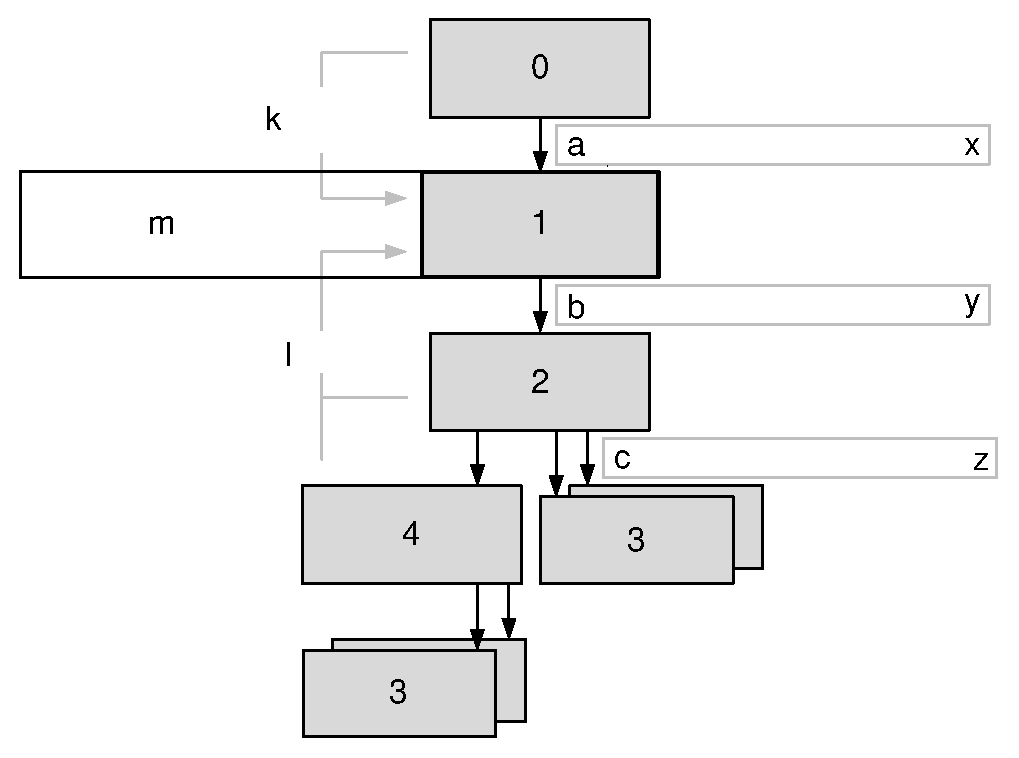
\includegraphics[width=1.\textwidth,clip, trim = 0cm 0cm 0cm 0cm]{2_KOS.eps}
 \caption[Beispielhafte Baumstruktur der Koordinatensysteme]{Beispielhafte Baumstruktur der Koordinatensysteme zur Entkopplung von lokalen und globalen Messinformationen}
 \label{fig:KOS}
\end{figure} 

Der große Vorteil dieser Trennung von lokalen und globalen Koordinatensystemen liegt nun darin, dass sich die für die globale Lokalisierung typischen Korrektursprünge der Position und Ausrichtung (Tunnelende bei GPS, Auftauchen von neuen Landmarken bei Video) nur auf das Optimierungskriterium (Wo möchte ich \emph{langfristig} hinfahren?) auswirken, nicht jedoch unmittelbar auf die Fahrzeugregelung und Hindernisprädiktion. Letztere werden nämlich in lokalen, aufintegrierten und damit sprungfreien Koordinaten durchgeführt und profitieren dabei von der kurzen Zykluszeit der Koppelnavigation (z.B.\ $\unit[10]{ms}$).
%. Darüber hinaus reicht es aus, eine globale Positionsschätzung mit einer niedrigen Frequenz zur Verfügung zu stellen, da aufgrund der schnellen Inertialsensorik eine sehr kurze Zykluszeit realisiert werden kann. 
Fällt gar die globale Lokalisierung ganz weg, so muss lediglich auf die global referenzierte Zusatzinformation im Fahrerassistenzsystem verzichtet werden, nicht jedoch auf die restliche Funktionalität.

%\section{Herleitungen und Beweise}
\section{Rekursive Lösbarkeit und Stabilität der MPC} \label{app:mpc_zielregion}
\begin{figure}[h]
\centering
    \psfrag{0}[ct][ct][1.]{$\bs x(t_k)$}
		\psfrag{z}[bl][bl][1.]{$\bar{\bs x}^\ast(t_k\!+\!\Delta t;\bs x(t_k))$}
    \psfrag{x}[tr][tr][1.]{$\bar{\bs x}^\ast(\tau;\bs x(t_k))$}
		\psfrag{n}[tr][tr][1.]{$\tilde{\bs x}(\tau)$}
		\psfrag{X}[cc][cc][1.]{$\mathcal X_f$}
		\psfrag{D}[bc][bc][1.]{$\Delta t$}
		\psfrag{T}[bc][bc][1.]{$T$}
		\psfrag{r}[bl][bl][1.]{$\bar{\bs x}_r(\tau)$}
		\psfrag{t}[tc][tc][1.]{$t,\tau$}
		\psfrag{1}[tc][tc][.9]{$t_{k}$}
		\psfrag{2}[tc][tc][.9]{$t_{k}\!+\!\Delta t$}
		\psfrag{3}[tc][tc][.9]{$t_{k}\!+\!T$}
		\psfrag{4}[tc][tc][.9]{$t_{k} \!+\! \Delta t\!+\!T$}
	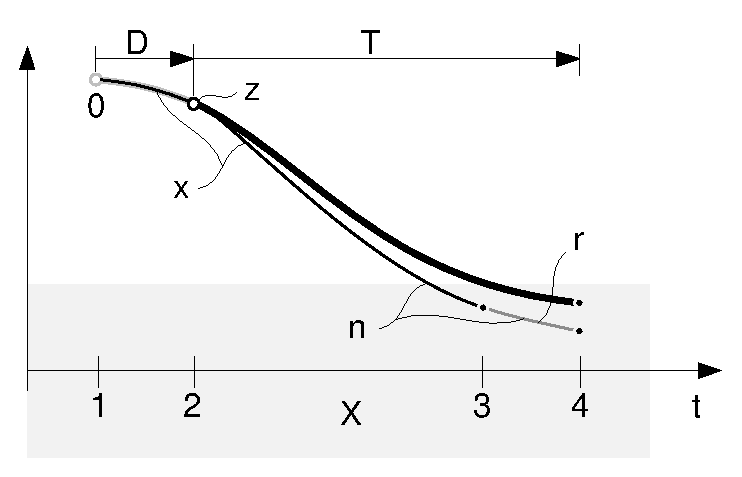
\includegraphics[width=.85\textwidth,clip, trim = 0cm 0cm 0cm 0cm]{3_mpc_jyapunov.eps}
	\caption[Stabilitätsbeweis der modellprädiktiven Regelung]{Veranschaulichung des Stabilitätsbeweises der modellprädiktiven Regelung mit Zielregion und -kosten, vgl.\ \cite{graichen2014SkriptOpt}}
	\label{fig:mpc_jyapunov}
\end{figure}
Entsprechend der Herleitung in \cite{graichen2014SkriptOpt}  seien zwei aufeinanderfolgende Zeitpunkte $t_k$ und $t_k\!+\!\Delta t$ betrachtet. In Abb.\,\ref{fig:mpc_jyapunov} ist die für einen Anfangszustand $\bs x(t_k)$ auf dem endlichen Horizont optimale Trajektorie $\bar{\bs x}^\ast(\tau,\bs x(t_k))$, $\tau \in [t_k, t_k \!+\! T]$ mit einer dünnen schwarzen Linie eingezeichnet. Das MPC-Stellgesetz führt also das System über einen Zeitschritt $\Delta t$ in den Zustand $\bar{\bs x}^\ast(t_k\!+\!\Delta t,\bs x(t_k))$ über. Dieser stellt den Anfangszustand für den nächsten Optimierungsschritt dar, dessen Lösungstrajektorie als dicke schwarze Linie eingezeichnet ist. Eine entsprechend der Nebenbedingungen zulässige Trajektorie ist $\tilde{\bs x}(\tau)$, $\tau \in [t_k\!+\!\Delta t, t_k\!+\!\Delta t + T]$.  Sie setzt sich aus dem hinteren Teil $\bar{\bs x}^\ast(\tau,\bs x(t_k))$ $\tau \in [t_k\!+\!\Delta t, t_k + T]$ der optimalen Trajektorie des vorherigen Optimierungsschritts und der Trajektorie $\bar{\bs x}_r(\tau)$, $\tau \in (t_k\!+T, t_k\!+\!\Delta t + T]$ zusammen, die sich durch Anwendung des lokalen Regelgesetzes $\bar{\bs u}(\tau) = \bs r(\bar{\bs x}_r(\tau))$ ergibt. Letztere ist durch eine dünne graue Linie dargestellt. Es gilt nun immer 
\begin{align} \label{app:ungl}
	J^\ast(\bs x^\ast(t_k \!+\! \Delta t; \bs x(t_k))) \leq J(\tilde{\bs x}(\tau),\tilde{\bs u}(\tau)) \; , 
\end{align}
da die optimalen Kosten $J^\ast$ nie größer, als die der zusammengesetzten Trajektorie $\tilde{\bs x}(\tau)$ sein können. Die Ungleichung \eqref{equ:mpc_control_lyapunov_ungl} kann nun umgeschrieben werden zu 
\begin{align}
	\frac{\rm d}{{\rm d} \tau} V(\bar{\bs x}_r(\tau))  + l(\bar{\bs x}_r(\tau), \bar{\bs u}_r(\tau)) \leq 0\;, \label{app:ungl_Lyap}
\end{align}
womit sich die rechte Seite von \eqref{app:ungl} als
\begin{align*}
	 J(&\tilde{\bs x}(\tau),\tilde{\bs u}(\tau)) = J^\ast(\bs x(t_k)) - \int_{t_k}^{t_k+\Delta t} \!\!\!\! l(\bar{\bs x}^\ast(\tau; \bs x(t_k)), \bar{\bs u}^\ast(\tau; \bs x(t_k))){\rm d} \tau \\
	&+ \underbrace{V(\bar{\bs x}_r(t_k \!+\! \Delta t \!+\! T)) - V(\bar{\bs x}_r(t_k \!+\! T)) + \int_{t_k \!+\! T}^{t_k + \Delta t \!+\! T} \!\!\!\! \!\!\! l (\bar{\bs x}_r(\tau),\bar{\bs u}_r(\tau)){\rm d}{\tau}}_{\leq 0}
\end{align*}
darstellen lässt. Der unterklammerte Ausdruck ist nicht-positiv, da er das Integral von \eqref{app:ungl_Lyap} ist. Insgesamt ergib sich somit aus \eqref{app:ungl}
\begin{align*}
	J^\ast(\bs x^\ast(t_k \!+\! \Delta t; \bs x(t_k))) \leq J^\ast(\bs x(t_k)) - \!\!\!\! \int_{t_k}^{t_k+\Delta t} \!\!\!\! l(\bar{\bs x}^\ast(\tau; \bs x(t_k)), \bar{\bs u}^\ast(\tau; \bs x(t_k))){\rm d} \tau
\end{align*}
was in Gleichheit dem unendlichen Optimierungshorizont entspricht und analog hierzu Stabilität garantiert \cite{graichen2014SkriptOpt}.

\section{Herleitung der Anhängergierdynamik} \label{app:herleitung_anhaengerdynamik}
Zur Herleitung wird der Geschwindigkeitsvektor $\boldsymbol v_c$ vom Kupplungspunkt  $\boldsymbol r_c$ mit Versatz $l_c>0$ zur Hinterachse herangezogen. Zunächst wird dieser aus Sicht des Zugfahrzeugs unter Zuhilfenahme dessen Gierratenvektors $\boldsymbol\omega_v=[0,\,0,\,\dot\psi_v]^\T$ und Geschwindigkeitsvektors $\boldsymbol v_v = [v_x, v_y, 0]^\T_v$ betrachtet, wodurch sich mit der Mittelpunktposition $\boldsymbol r_v$ von der Zugfahrzeughinterachse der Zusammenhang
\begin{align} \nonumber
	\boldsymbol v_c &= \boldsymbol v_v+\boldsymbol\omega_v\times\left[\boldsymbol r_c-\boldsymbol r_v\right] \\
	&= \begin{bmatrix}v_v\cos\psi_v\\v_v\sin\psi_v\\0\end{bmatrix}+\begin{bmatrix}0\\0\\\dot\psi_v\end{bmatrix}\times\begin{bmatrix}-l_c\cos\psi_v\\-l_c\sin\psi_v\\0\end{bmatrix}\label{eq:fzgmodell:vc_von_vv}
\end{align}
ergibt. Analog wird mit dem Gierratenvektor $\boldsymbol\omega_t=[0,\,0,\,\dot\psi_t]^\T$, dem  Achsmittelpunkt $\boldsymbol r_t$ mit Geschwindigkeitsvektor $\boldsymbol v_t$  und der Deichsellänge~$l_t>0$ des Anhängers
\begin{align} \nonumber
	\boldsymbol v_c &= \boldsymbol v_t+\boldsymbol\omega_t\times\left[\boldsymbol r_c-\boldsymbol r_t\right] \\
	&= \begin{bmatrix}v_t\cos\psi_t\\v_t\sin\psi_t\\0\end{bmatrix}+\begin{bmatrix}0\\0\\\dot\psi_t\end{bmatrix}\times\begin{bmatrix}l_t\cos\psi_t\\l_t\sin\psi_t\\0\end{bmatrix}\label{eq:fzgmodell:vc_von_vt}
\end{align}
erhalten. Gleichsetzen von \eqref{eq:fzgmodell:vc_von_vv} mit \eqref{eq:fzgmodell:vc_von_vt} liefert mit \eqref{eq:fzgmodell:psi_v_dot} unter Zuhilfenahme der Additionstheoreme die gesuchte Anhängergierdynamik \eqref{eq:fzgmodell:psi_t_dot} sowie die vorzeichenbehaftete Anhängergeschwindigkeit \eqref{eq:fzgmodell:v_t}.

%\section{Verzugskompensation}
%Da das ausweichende Fahrzeug innerhalb eines Sekundenbruchteils eine erhebliche Strecke zurücklegt, können die erforderlichen Optimierungszykluszeiten nicht vernachlässigt werden. Aus diesem Grund wird eine Verzugskompensation mittels Prädiktion (engl.\ \emph{delay compensation by prediction} \cite{diehl_numerical_methods}) durchgeführt. 


%\section{Programmbeispiele}

%Seitenübersicht:

%1. Kap:  5
%2. Kap: 45
%3. Kap: 40  --> 20 + 20 Anhänger
%4. Kap: 26  --> 14 + 12 NMPC
%5. Kap: 30  --> 15 + 15 Riccati
%6. Kap: 10
%7. Kap:  5
%tot:   161
%\section{Beispielhafte Programmstruktur der direkten Optimierung}
%\begin{figure}[ht] 
	%%\vspace{0.3cm}
	%\psfrag{1}[c][c][1.0]{Berechnung der optimalen Stellgröße}	
	%%\psfrag{1}[c][c][1.0]{\parbox[t]{15cm}{\begin{center}Berechnung der optimalen Trajektorie\\ \textbf{solveOCP()}\end{center}}}
	%\psfrag{2}[c][c][1.0]{\parbox[t]{5cm}{\begin{center}Optimierung\\ der \\ Stellgröße $\bar{\bs{u}}$\\ mit Hilfe \\ eines \\ SQP-Verfahrens \end{center}}}
	%\psfrag{3}[c][c][1.0]{\parbox[t]{7cm}{\begin{center}Berechnung \\ der \\Trajektorienkosten \end{center}}}
	%\psfrag{4}[c][c][1.0]{\parbox[t]{5cm}{\begin{center}Prädiktion des \\Systemzustandes \\ mittels ODE-Solver\end{center}}}
	%\psfrag{5}[c][c][1.0]{\parbox[t]{7cm}{\begin{center}Berechnung \\ der \\Nebenbedingung \end{center}}}
	%\psfrag{6}[c][c][1.0]{$\xi_\text{num}$}
	%\psfrag{X}[c][c][1.0]{$\bs{x}_{0}$}
	%\psfrag{O}[c][c][1.0]{Hindernis}
	%\psfrag{U}[c][c][1.0]{$\bs{\bar x}$}
	%\psfrag{x}[c][c][1.0]{$\bar{\bs{x}}$}
	%\psfrag{u}[c][c][1.0]{$\bar{\bs{u}}$}
	%\psfrag{g}[c][c][1.0]{$\bs{h}(\bar{\bs{u}};\bs{x}_{0}, \gamma)$}
	%\psfrag{J}[c][c][1.0]{$J(\bar{\bs{u}}; \bs{x}_0)$}
	%\hspace{0.3cm}
%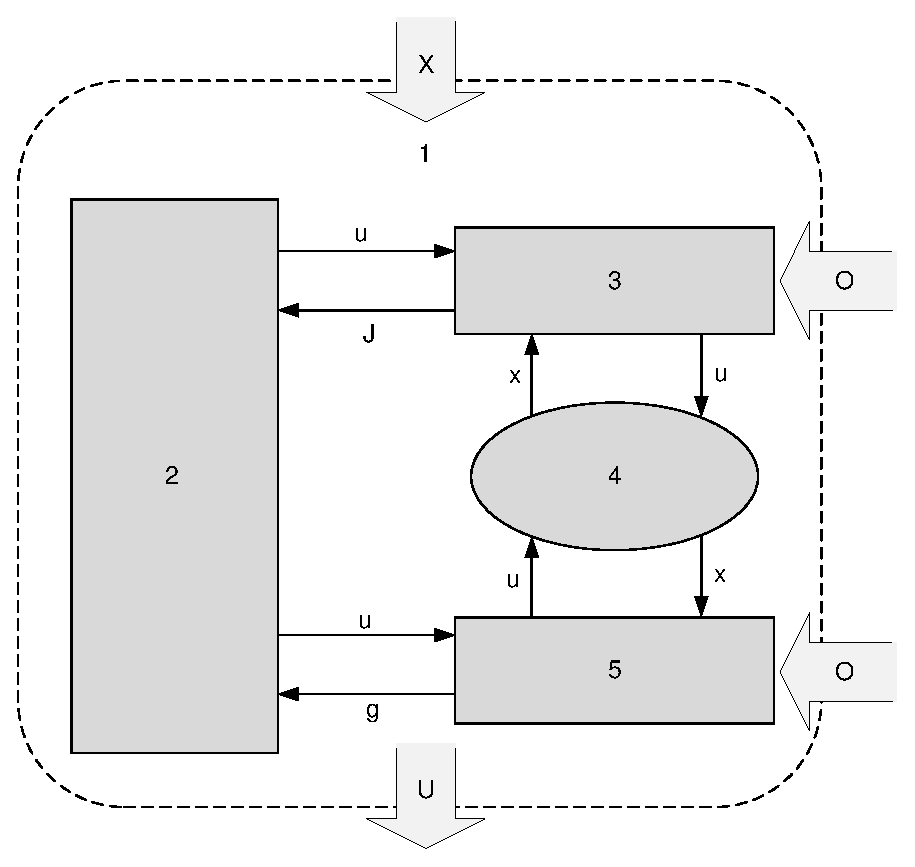
\includegraphics[width=.95\textwidth,clip, trim = 0cm 0cm 0cm 0cm]{_opti_solveOCP-ablaufplan.eps}
	%\ \vspace{-0.2cm}
%\caption[MPC Programmablauf mit SQP-Verfahren]{Veranschaulichung des Programmablaufs zur Berechnung der optimalen Ausweichtrajektorie mittels SQP-Verfahrens}
%\label{fig:solveOCP_ablaufplan}
%\end{figure}    

%\addtocontents{toc}{\protect\setcounter{tocdepth}{3}}% standard
